%%%%%%%%%%%%%%%%%%%%%%%%%%%%%%%%%%%%%%%%%
% University/School Laboratory Report
% LaTeX Template
% Version 3.1 (25/3/14)
%
% This template has been downloaded from:
% http://www.LaTeXTemplates.com
%
% Original author:
% Linux and Unix Users Group at Virginia Tech Wiki 
% (https://vtluug.org/wiki/Example_LaTeX_chem_lab_report)
%
% License:
% CC BY-NC-SA 3.0 (http://creativecommons.org/licenses/by-nc-sa/3.0/)
%
%%%%%%%%%%%%%%%%%%%%%%%%%%%%%%%%%%%%%%%%%

%----------------------------------------------------------------------------------------
%	PACKAGES AND DOCUMENT CONFIGURATIONS
%----------------------------------------------------------------------------------------

\documentclass[scale = 0.9]{article}
\usepackage[a3paper, total={10in, 15in}]{geometry}

\usepackage[T1]{fontenc}
\usepackage{lmodern}
 
\usepackage[version=3]{mhchem} % Package for chemical equation typesetting
\usepackage{siunitx} % Provides the \SI{}{} and \si{} command for typesetting SI units
\usepackage{graphicx} % Required for the inclusion of images
\usepackage{natbib} % Required to change bibliography style to APA
\usepackage{amsmath} % Required for some math elements 

\usepackage[hidelinks]{hyperref}

\setlength\parindent{0pt} % Removes all indentation from paragraphs

\renewcommand{\labelenumi}{\alph{enumi}.} % Make numbering in the enumerate environment by letter rather than number (e.g. section 6)

%\usepackage{times} % Uncomment to use the Times New Roman font

\usepackage{float}

\usepackage{enumitem}

\usepackage{xcolor}
\definecolor{light-gray}{gray}{0.95}

\let\oldsection\section
\renewcommand\section{\clearpage\oldsection}

\newcommand{\code}[1]{\colorbox{light-gray}{\texttt{#1}}} % change a string to coding font.
%----------------------------------------------------------------------------------------
%	DOCUMENT INFORMATION
%----------------------------------------------------------------------------------------

\title{Report \\ TETRIS \\ Built for De1\_SoC device} % Title

\author{Khang \textsc{Phan}} % Author name

\date{\today} % Date for the report

\begin{document}

\maketitle % Insert the title, author and date

% If you wish to include an abstract, uncomment the lines below
% \begin{abstract}
% Abstract text
% \end{abstract}

%----------------------------------------------------------------------------------------
%	SECTION 1
%----------------------------------------------------------------------------------------

\section{Overall design}
This is a tetris game using PS2 keyboard and VGA. Upon uploaded, press `N' for new game. 
Control using arrow keys, press PAUSE to hard drop, ESC to pause, `Z' and `X' to rotate 
counter clockwise and clock wise respectively. SW[9] is used to reset the screen display
if CLOCK\_74 is out of locked

Upon starting, a tetromino is generated. Each tetromino contains all of its possible 
rotation as well as current coordinate/rotation. The tetromino is spawned exactly above
the screen, row 0 and 1 respectively. Thus, this add up to internal row number to be
22 instead of just 20. The field is 22x10 grid, where each grid contains 4 bits to identify
which tetromino it form as well as the color of the tetromino block.
\subsection{Block diagram}
\begin{figure}[H]
  \begin{center}
    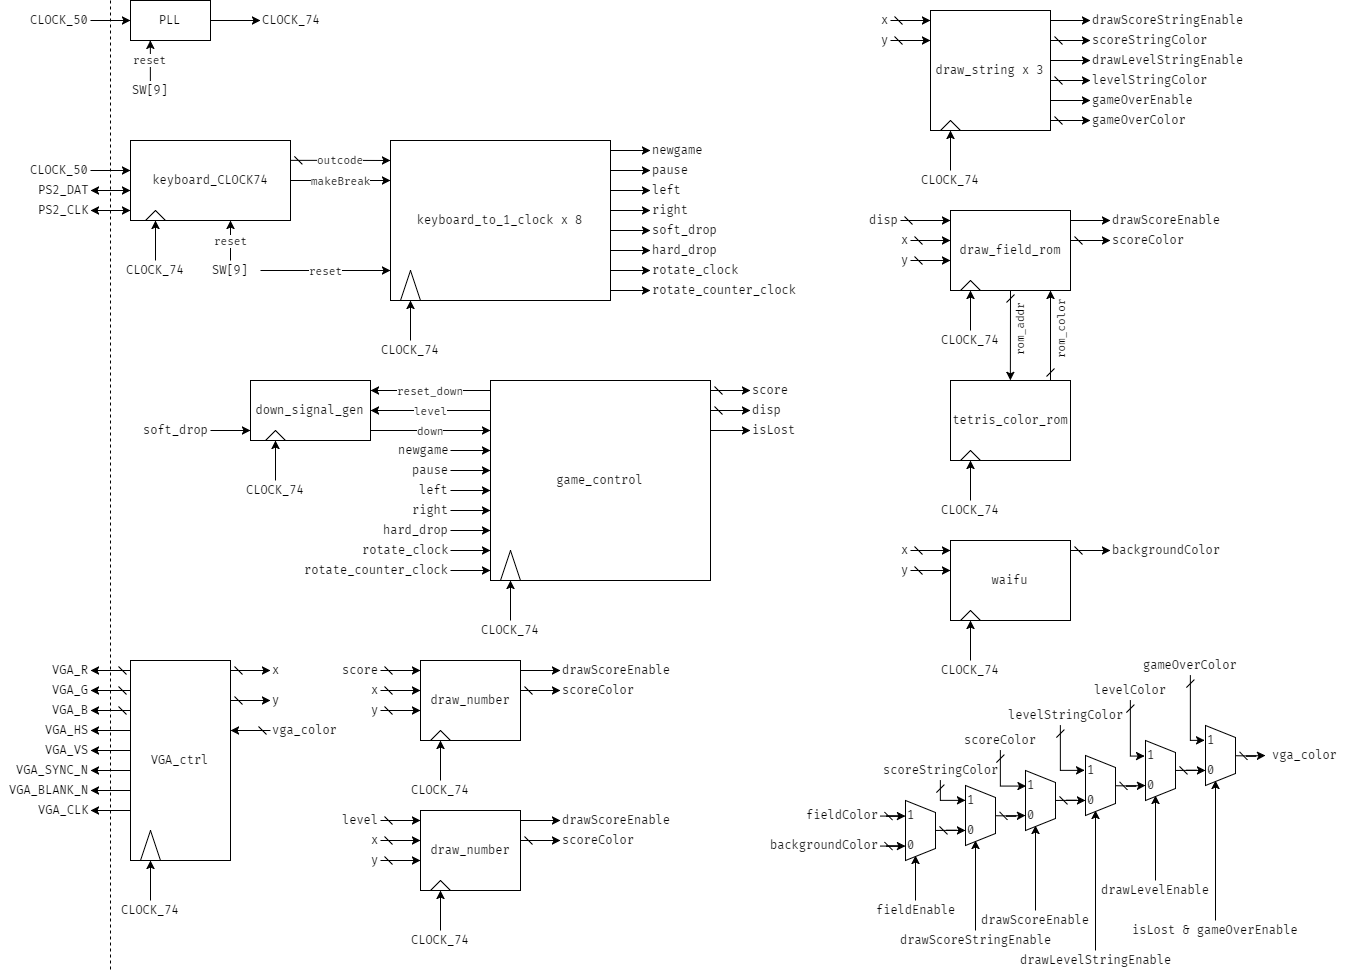
\includegraphics[width=\textwidth]{blockdiagram.png}
    \caption{High level block diagram}\label{blockdiagram}
  \end{center}
\end{figure}

The series of multiplexers is used with enable signal to decide which color to be drawn.
% TODO: add diagram

%----------------------------------------------------------------------------------------
%	SECTION 2
%----------------------------------------------------------------------------------------

\section{Modules}

\subsection{\code{create\_field}}

\begin{enumerate}[label=(\alph*)]
  \item Description:
        \code{create\_field} construct a tetris \code{field\_t} f\_out object by combining the origin
        \code{field\_t} f with the \code{tetromino\_ctrl} t\_ctrl being applied. The the data from
        t\_ctrl will overwrite f at any corresponding coordinate such that t\_ctrl has a block at.
        For example, the T tetromino that at coordinate (0,0) has the following rotation:
  \item Modelsim:

        This is the original \code{field\_t} f, note that only \code{111} means empty block:
        \begin{figure}[H]
          \begin{center}
            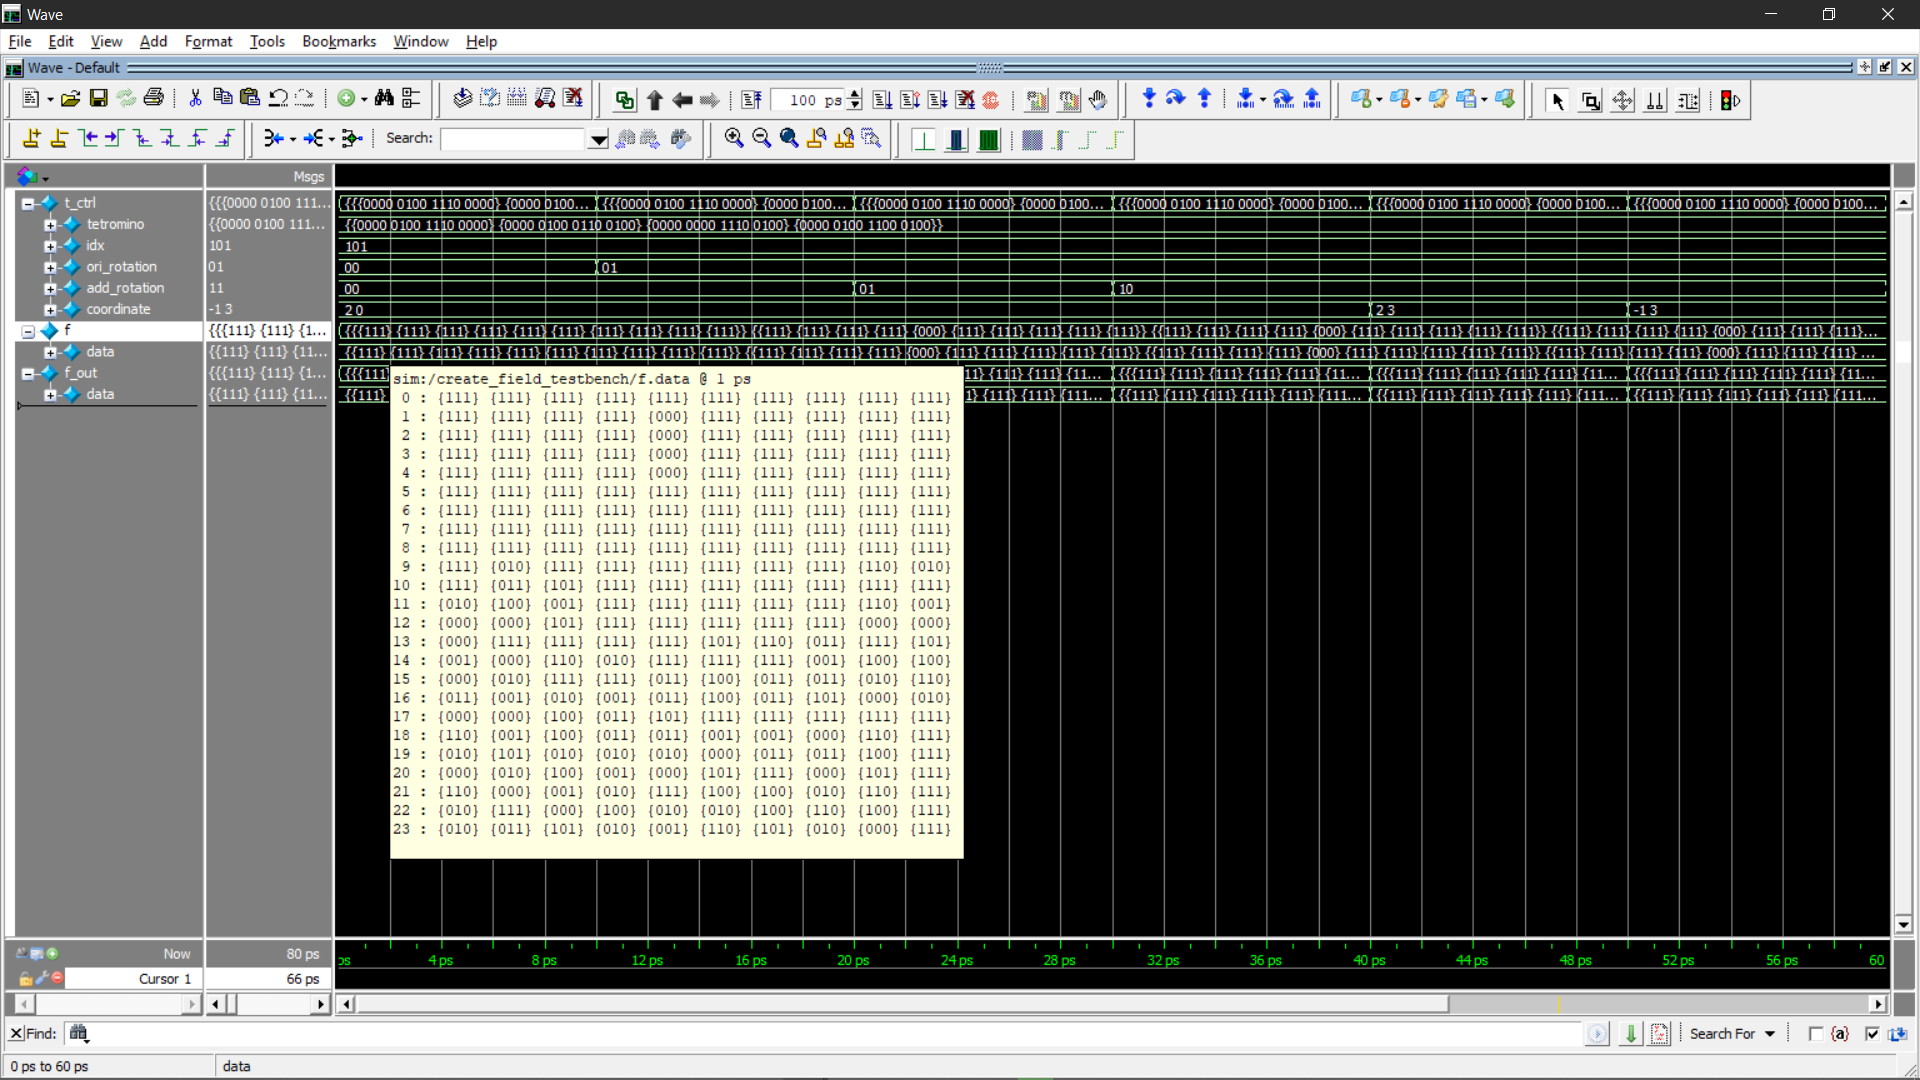
\includegraphics[width=0.9\textwidth]{create_field_1.png}
            \caption{\code{create\_field} modelsim 1}\label{create_field_1}
          \end{center}
        \end{figure}

        In this modelsim, my t\_ctrl is a T tetromino. It is at position (2,0) facing upward.
        After go through \code{create\_field} module, the result is as following:
        \begin{figure}[H]
          \begin{center}
            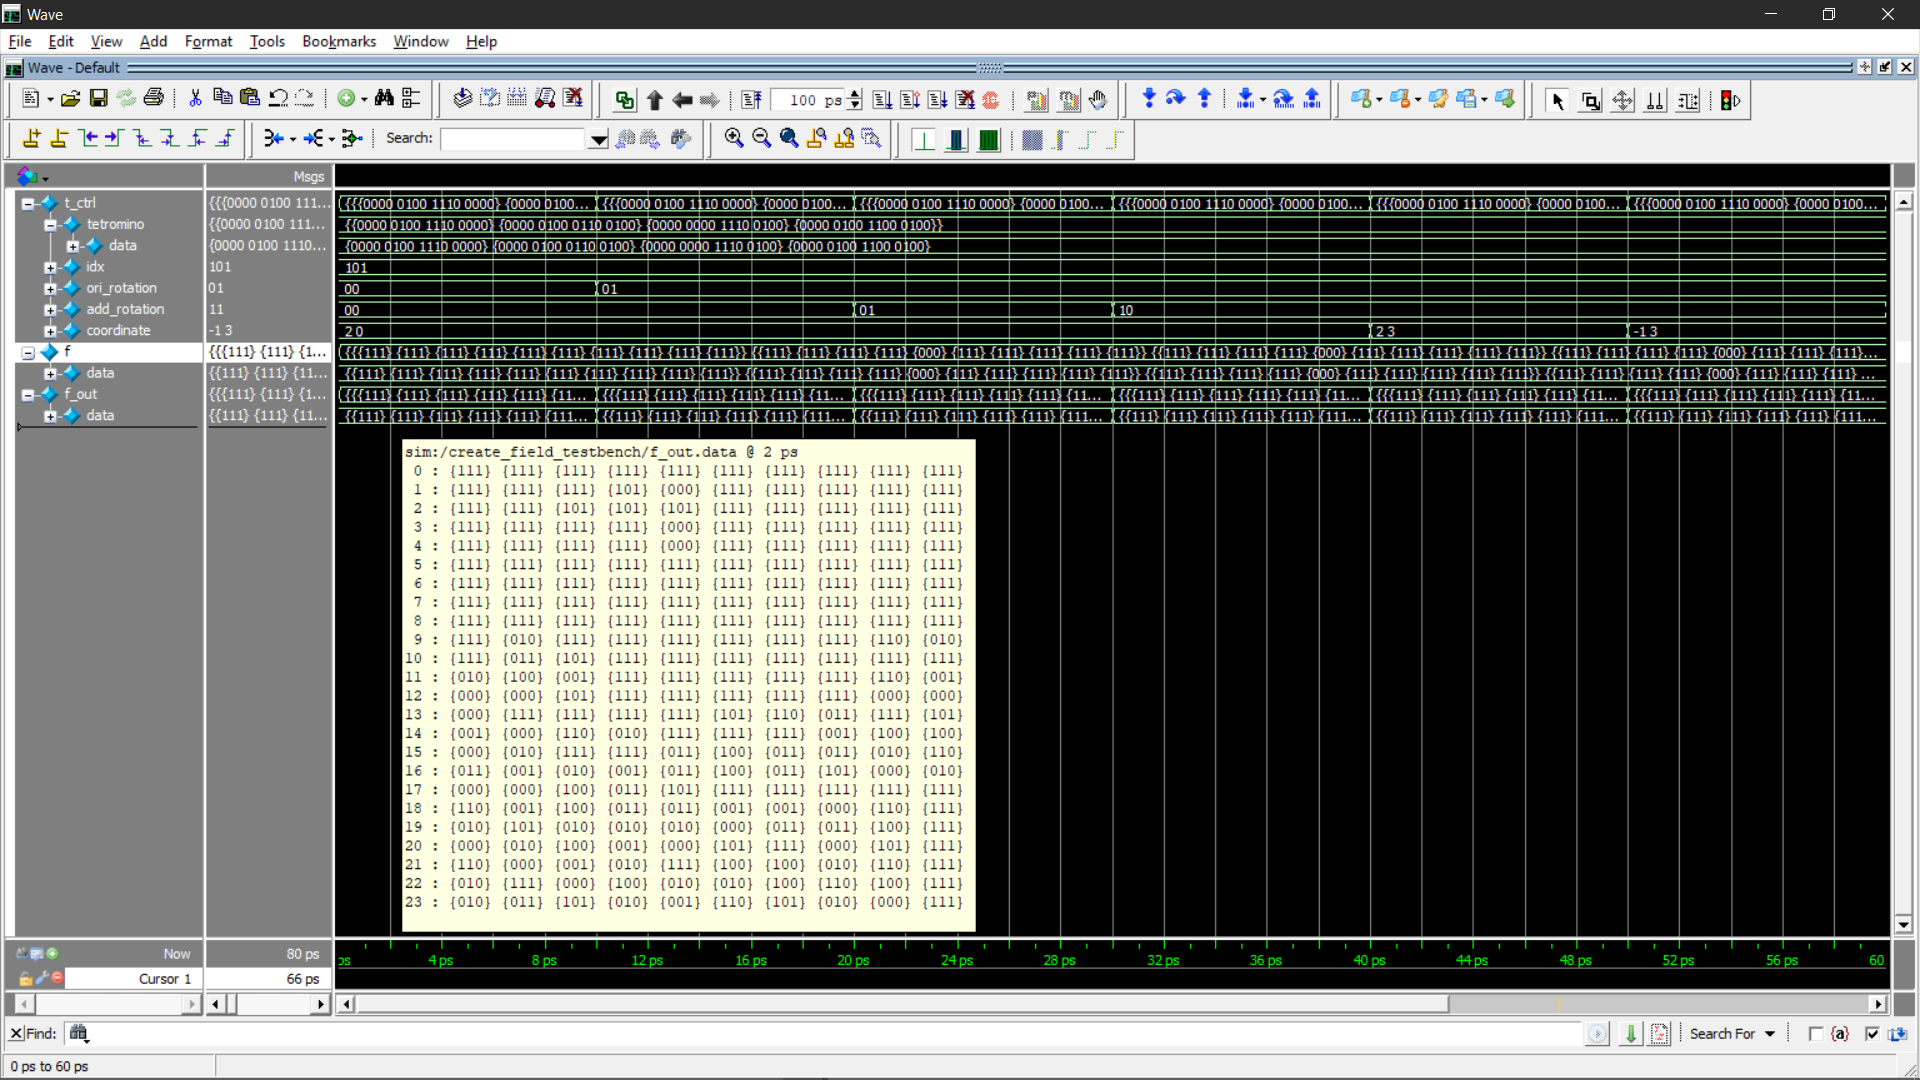
\includegraphics[width=0.9\textwidth]{create_field_2.png}
            \caption{\code{create\_field} modelsim 2}\label{create_field_2}
          \end{center}
        \end{figure}
        You can see in above that we have new \code{101} block that appear and even
        overwrite one original non empty \code{000} block. \code{101} is used to identify
        the T tetromino, also uses as color identifier for VGA display.

        Now I try to rotate the t\_ctrl:
        \begin{figure}[H]
          \begin{center}
            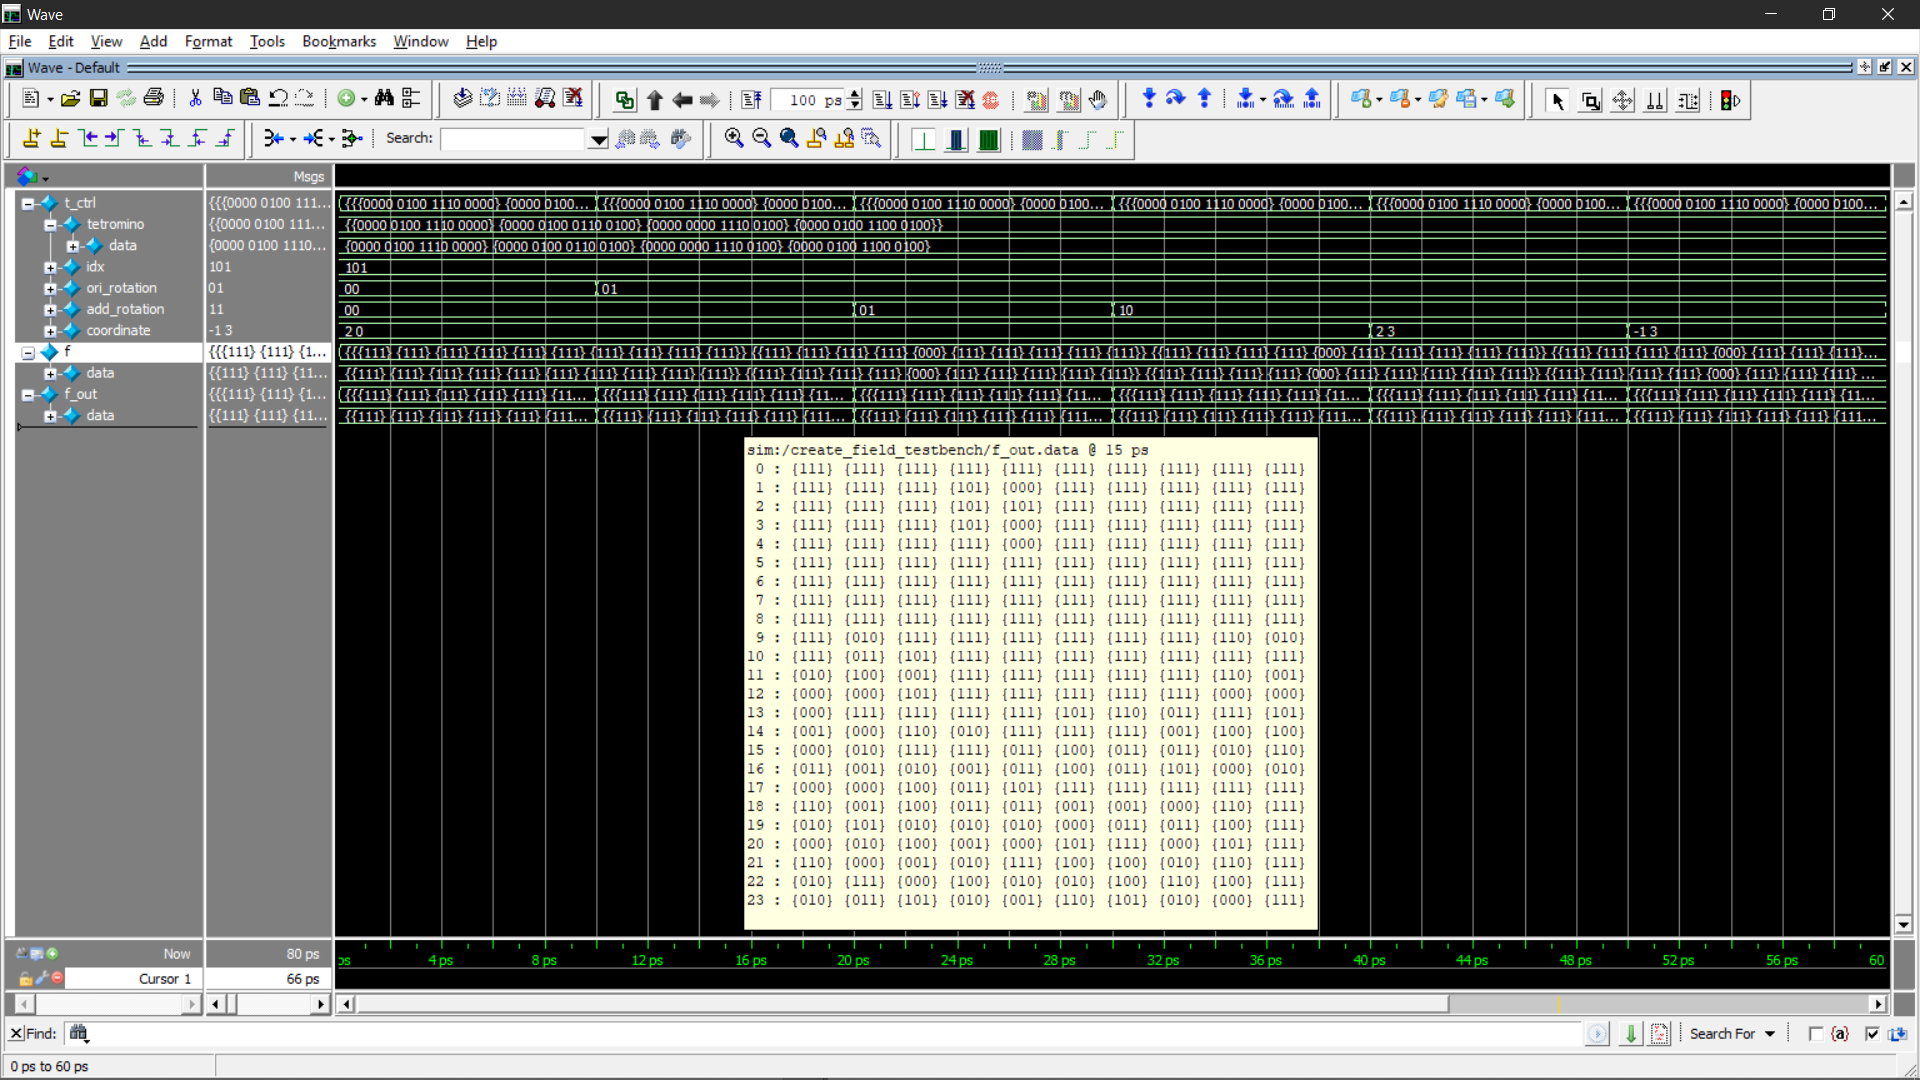
\includegraphics[width=0.9\textwidth]{create_field_3.png}
            \caption{\code{create\_field} modelsim 3}\label{create_field_3}
          \end{center}
        \end{figure}
        \begin{figure}[H]
          \begin{center}
            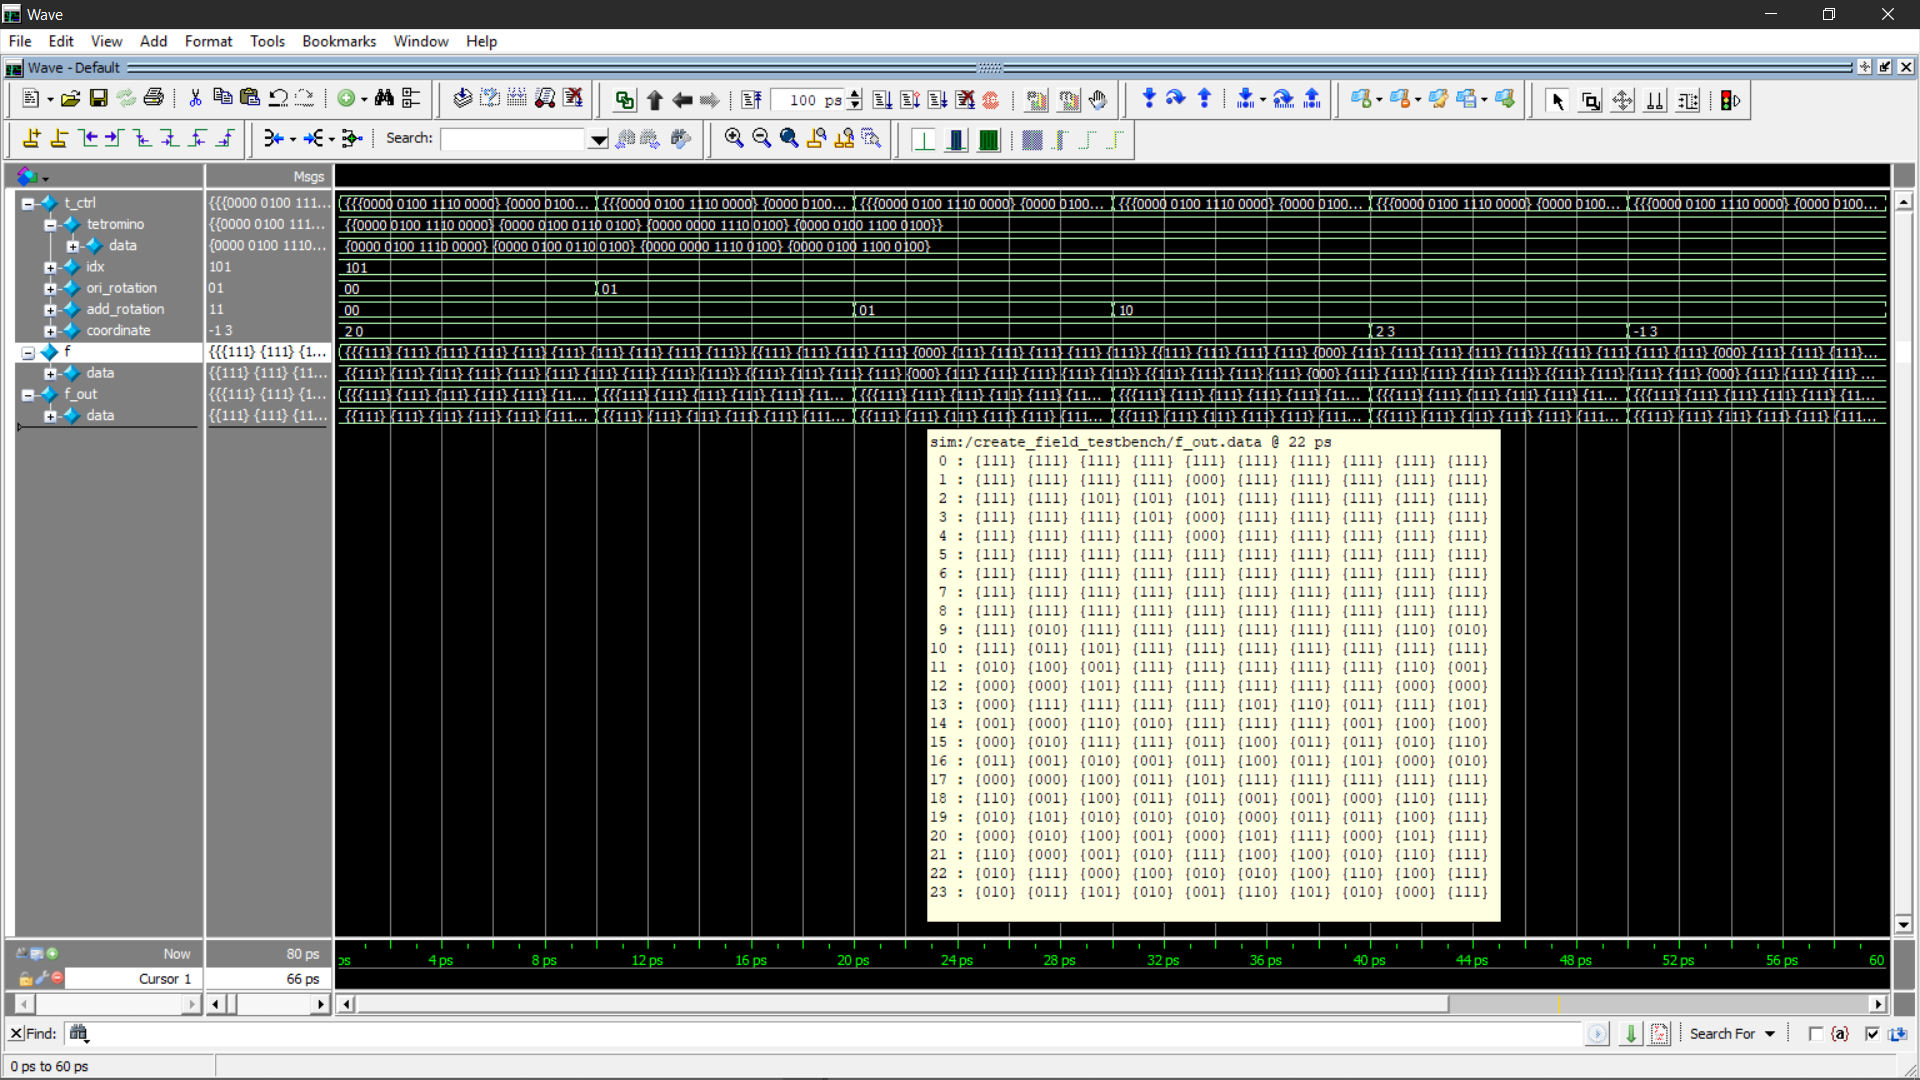
\includegraphics[width=0.9\textwidth]{create_field_4.png}
            \caption{\code{create\_field} modelsim 4}\label{create_field_4}
          \end{center}
        \end{figure}

        Even when I move the index of t\_ctrl to (-1, 3), you can see \code{101} block on the left size:
        \begin{figure}[H]
          \begin{center}
            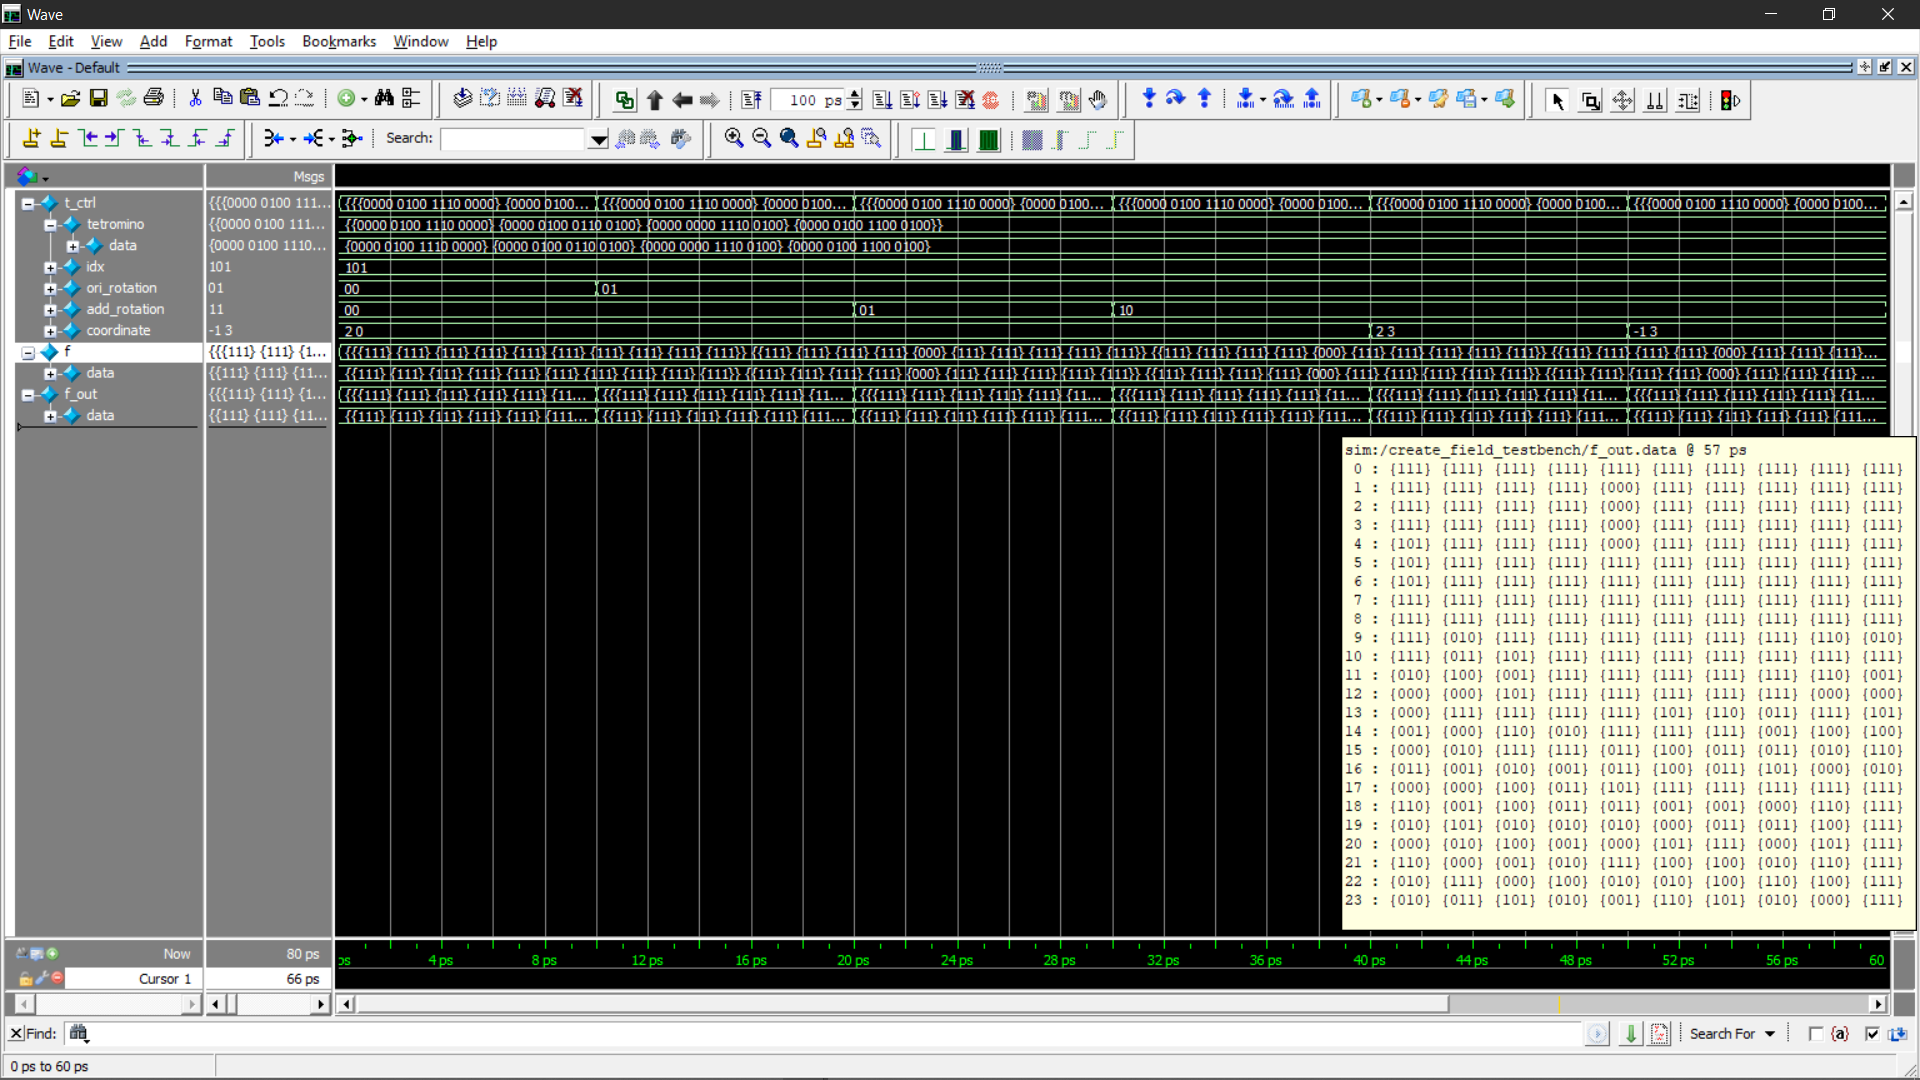
\includegraphics[width=0.9\textwidth]{create_field_5.png}
            \caption{\code{create\_field} modelsim 5}\label{create_field_5}
          \end{center}
        \end{figure}

\end{enumerate}

\subsection{\code{check\_valid}}
\begin{enumerate}[label=(\alph*)]
  \item Description:
        This module is slightly similar to \code{create\_field}, but instead of output a resulting field,
        it check if that field is valid or not. That means all \code{1} block of \code{tetromino\_ctrl}
        input must not be at a non empty block in \code{field\_t} input as well as not out of bound, i.e.
        not negative and less than the corresponding vertical/horizontal size.
  \item Modelsim:

        Using  the same input as \code{create\_field}'s testbench I got the following:
        \begin{figure}[H]
          \begin{center}
            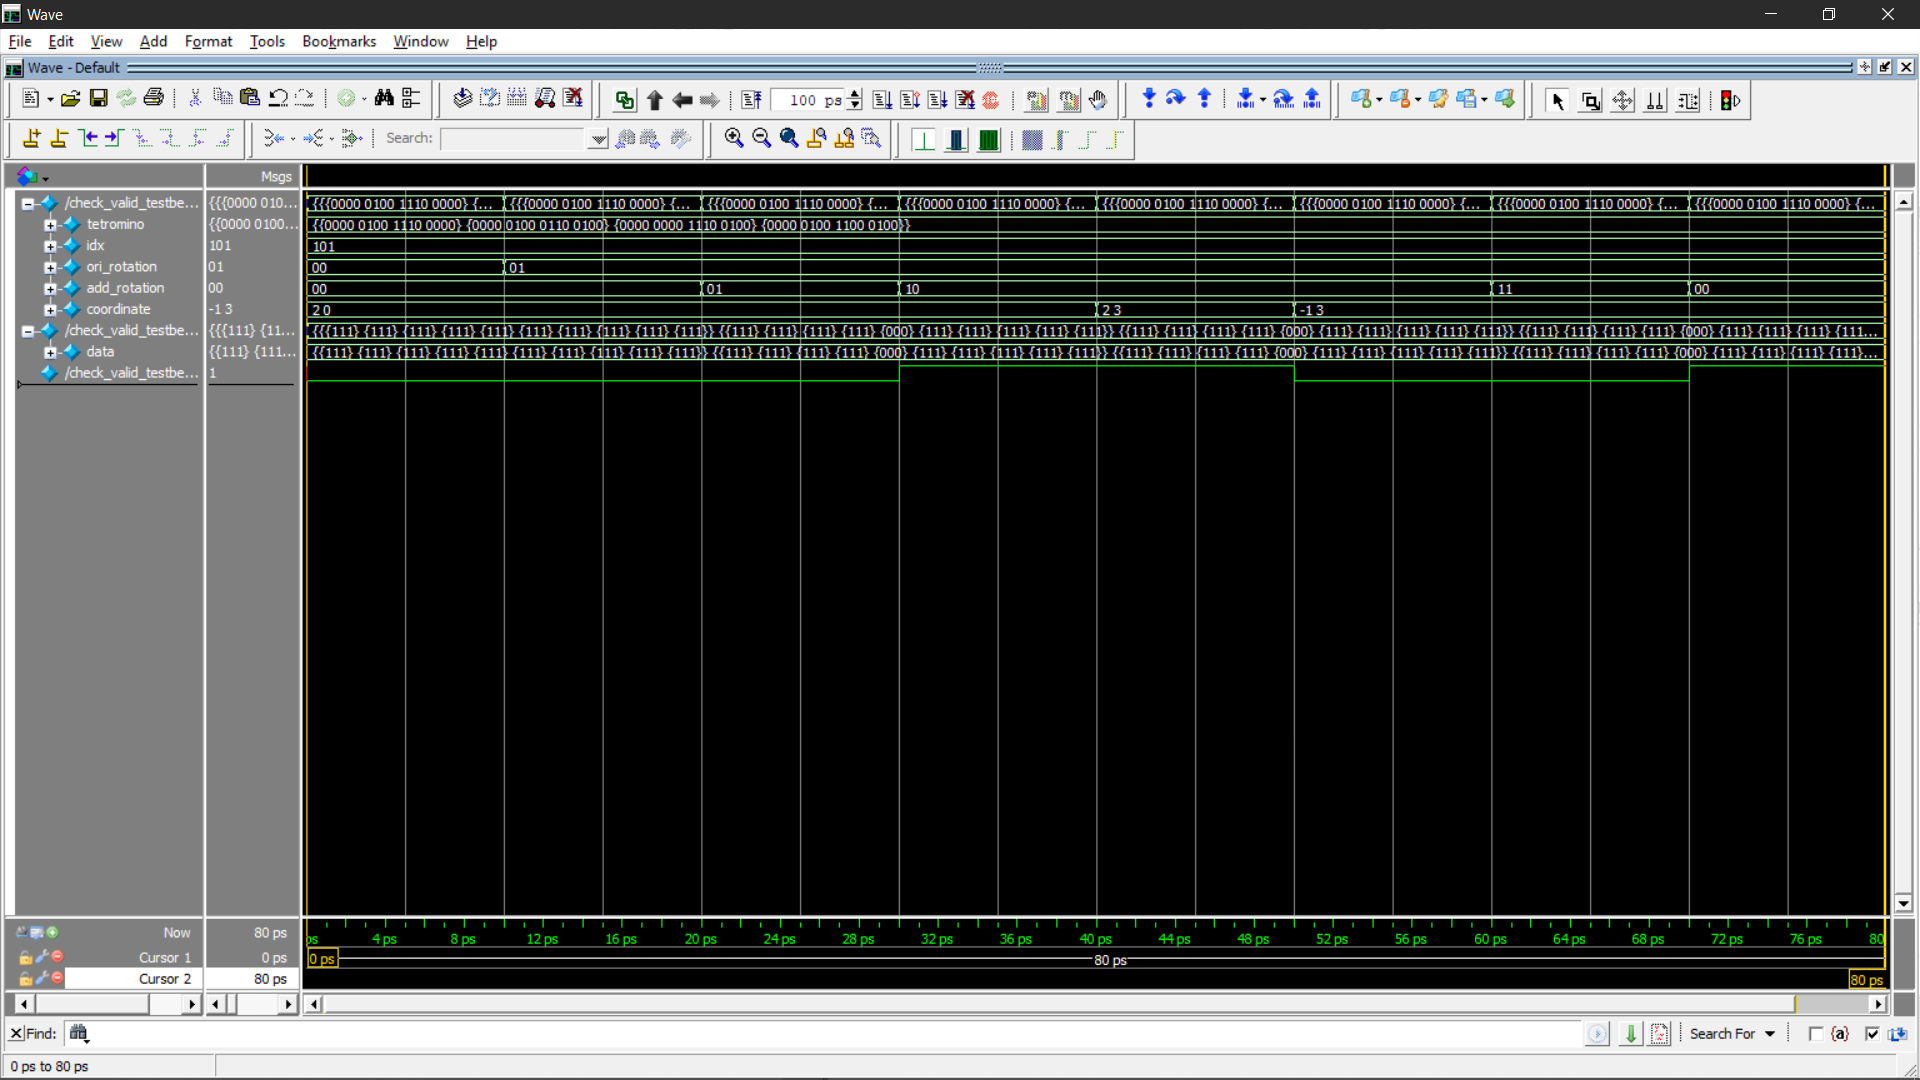
\includegraphics[width=0.9\textwidth]{check_valid.png}
            \caption{\code{check\_valid} modelsim}\label{check_valid}
          \end{center}
        \end{figure}

        You can see the first 3 states are not valid, this is the case of firgure \ref{create_field_2},
        \ref{create_field_3} and \ref{create_field_4} from \code{create\_field} testbench, this is not
        valid because the block overwrite the \code{000} in field, which is not allowed.

\end{enumerate}

\subsection{\code{clockwise\_wallkick\_data} and \code{counterclockwise\_wallkick\_data}}
\begin{enumerate}[label=(\alph*)]
  \item Description:
        These module get the additional x and y value to be added to coordinate for wall kicking.
        These value can be find on SRS wiki (\url{https://tetris.fandom.com/wiki/SRS}).
  \item Modelsim:

        The testbench is staight forward, where \code{000} idx represent I block:
        \begin{figure}[H]
          \begin{center}
            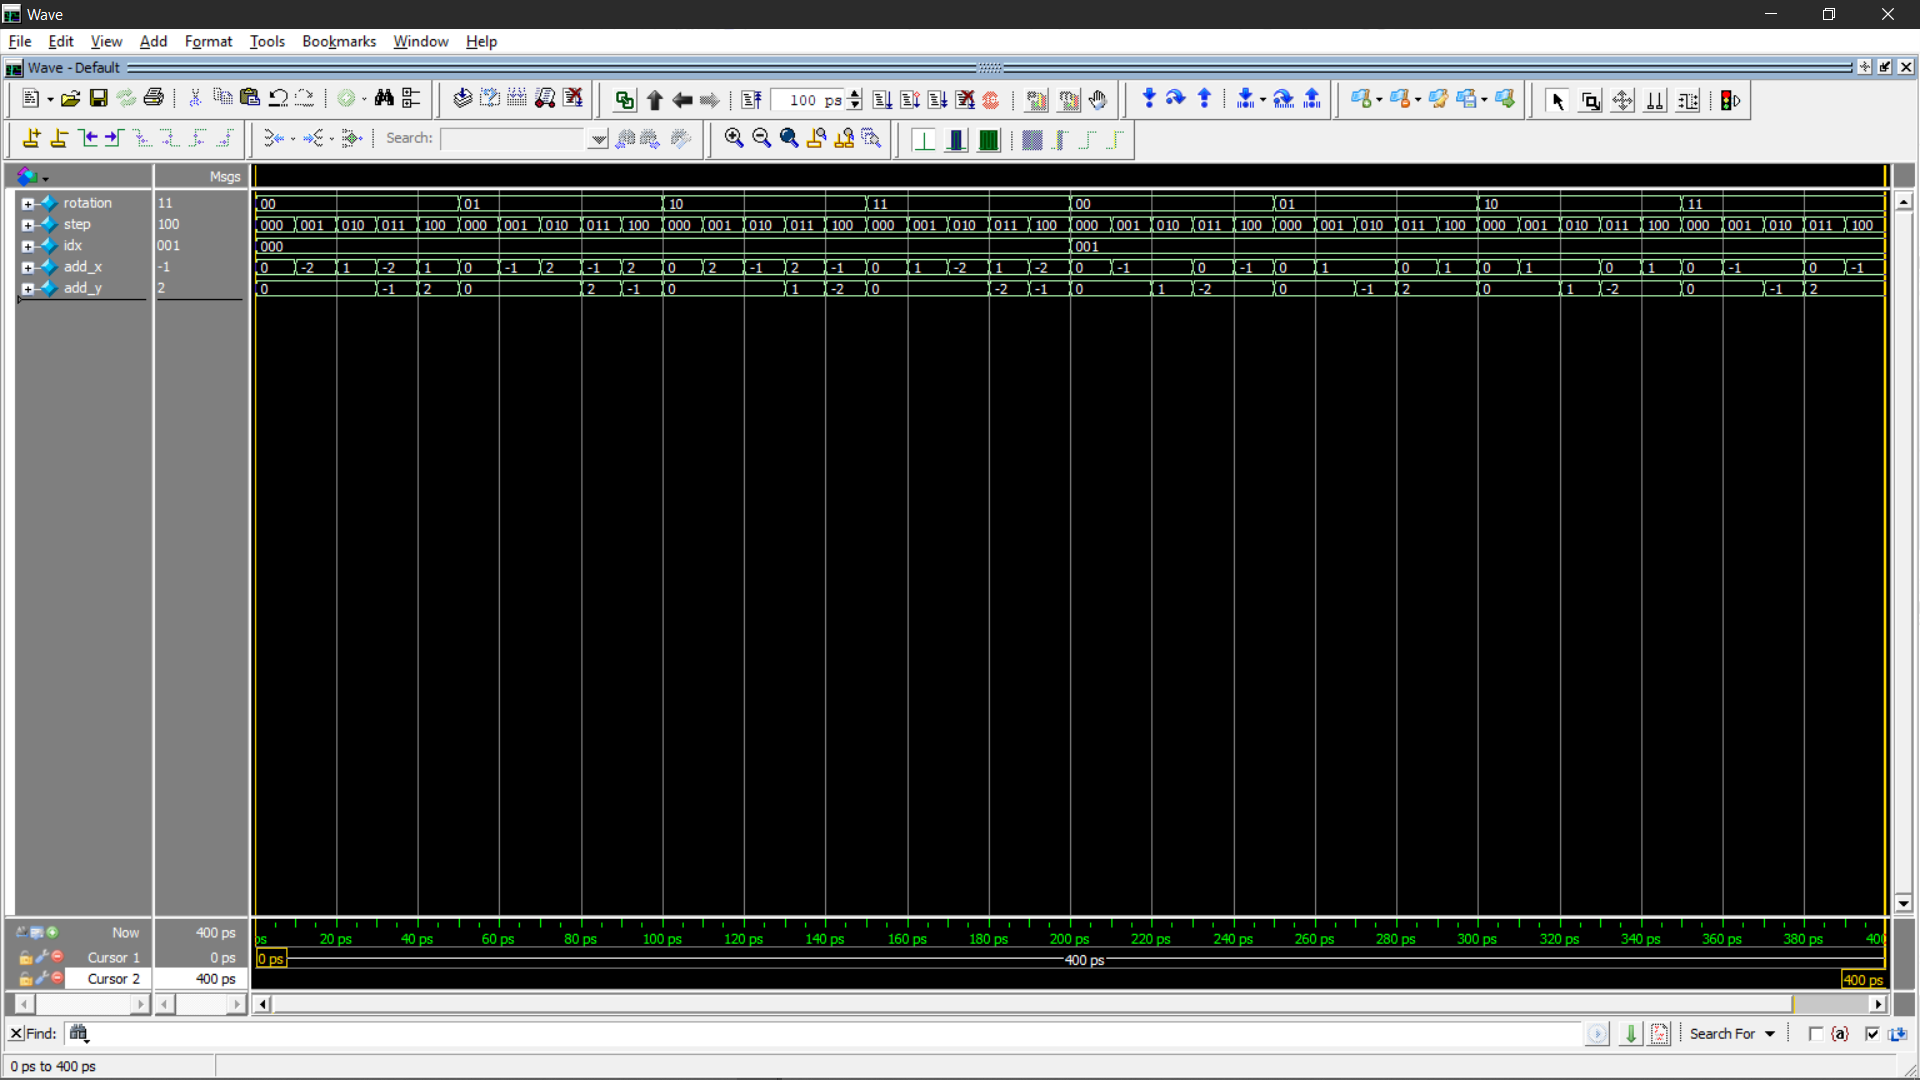
\includegraphics[width=0.9\textwidth]{clockwise_wallkick_data.png}
            \caption{\code{clockwise\_wallkick\_data} modelsim}\label{clockwise_wallkick_data}
          \end{center}
        \end{figure}

        Compare the result to the value on the wiki, these are all correct.

\end{enumerate}

\subsection{\code{rotate\_clockwise} and \code{rotate\_counterclockwise}}
\begin{enumerate}[label=(\alph*)]
  \item Description:
        These module take as most 5 clock and at least 1 clock to finish. How it works is simple. Each
        clock, it will propose a result rotated tetromino t\_out based on  the input tetromino t and
        add value in the corresponding \code{*\_wallkick\_data},
        if valid input is asserted that means it is accepted and will stay at that proposed value with done
        being output. If not, it will try the next propose, until it reach try5 state. At try5 state,
        done is always output, together with isFailed signal if valid is still false. This module
        only run when enable is high and reset once enable goes low.
  \item ASMD
        \begin{figure}[H]
          \begin{center}
            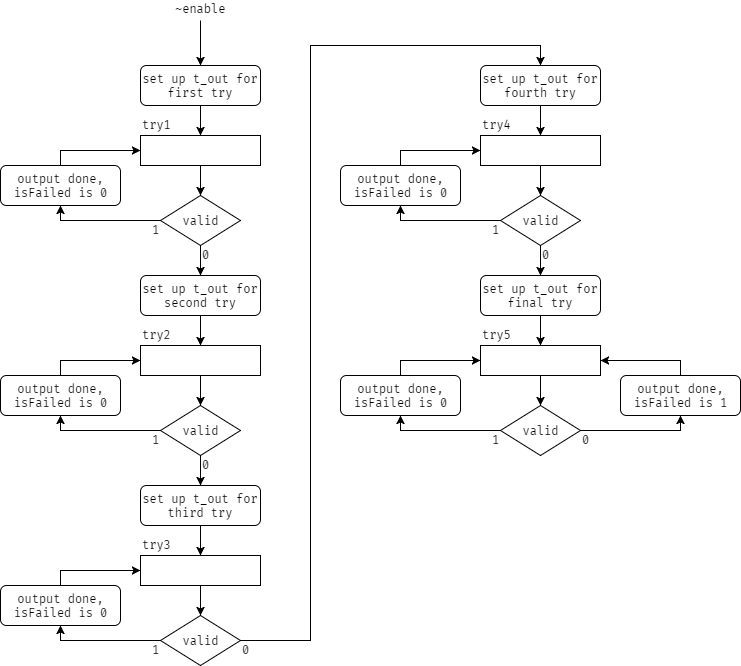
\includegraphics[width=0.7\textwidth]{rotate.png}
            \caption{\code{rotate\_clockwise} ASMD}\label{rotate_ASMD}
          \end{center}
        \end{figure}
  \item Modelsim:
        \begin{figure}[H]
          \begin{center}
            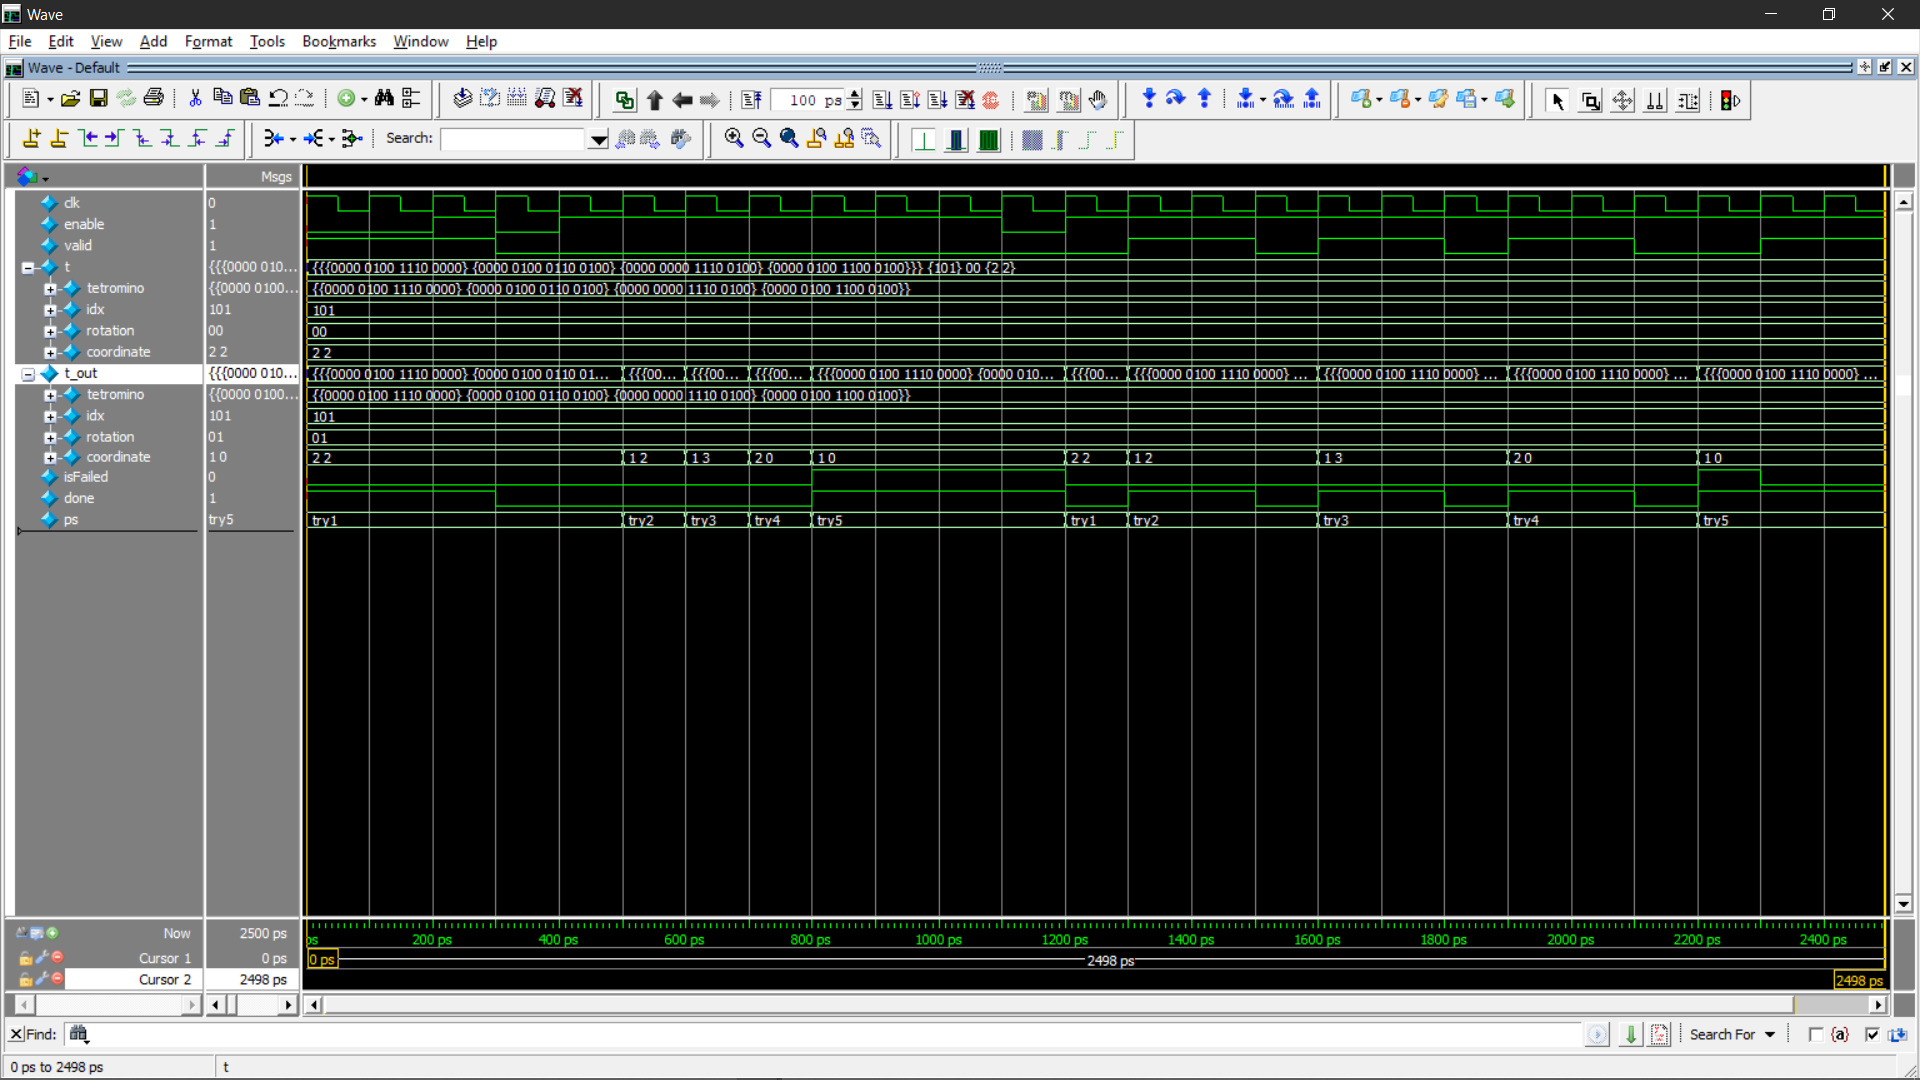
\includegraphics[width=0.9\textwidth]{rotate_clockwise.png}
            \caption{\code{rotate\_clockwise} modelsim}\label{rotate_clockwise}
          \end{center}
        \end{figure}

\end{enumerate}

\subsection{\code{generate\_tetromino}}
This module use LFSR to generate new tetromino. The number generated mod 7 is input
into \code{get\_tetromino\_info} module to output the correct tetromino and all its
rotation with initialized coordinate and rotation.

\subsection{\code{get\_tetromino\_info}}
This module output the corresponding tetromino based on he input index. Each tetromino
output is 4x4x4 bit, where [1][2][3] means tetromino block at rotation 1, y\_coordinate
2 and x\_coordinate 3. Thus, for T shape tetromino, it will look like this:

\begin{center}
  \code{0000}\\
  \code{0100}\\
  \code{1110}\\
  \code{0000}\\~\\


  \code{0000}\\
  \code{0100}\\
  \code{0110}\\
  \code{0100}\\~\\

  \code{0000}\\
  \code{0000}\\
  \code{1110}\\
  \code{0100}\\~\\

  \code{0000}\\
  \code{0100}\\
  \code{1100}\\
  \code{0100}
\end{center}





\subsection{\code{game\_control}}
\begin{enumerate}[label=(\alph*)]
  \item Description:
        This module handle game main logic. Depend on the signal input, the game will
        change to corresponding state. Note that even though there are different valid
        signal in the ASMD, they are all the same signal output from \code{check\_valid}
        module, only the input tetromino is different depend on the state.

        Another thing that is not mentioned in the ASMD is the isHardDrop signal. This
        signal went high when there is a hard\_drop input signal and stay high until
        state return to gen\_s. This create the effect that the block is drop down
        immediately and new block is generated.
  \item ASMD
        \begin{figure}[H]
          \begin{center}
            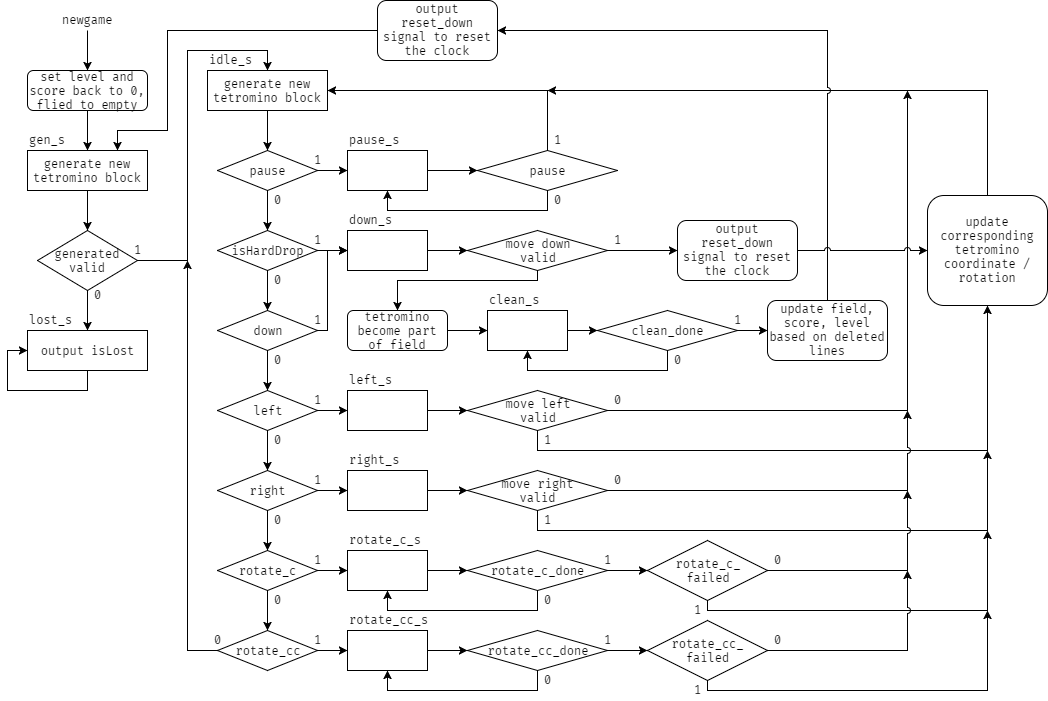
\includegraphics[width=\textwidth]{game_control.png}
            \caption{\code{game\_control} ASMD}\label{game_control_ASMD}
          \end{center}
        \end{figure}
\end{enumerate}

\subsection{\code{down\_signal\_gen}}
This module create a down signal based on a timer, when reset it will check current
level input and change back to the number to start count down from. It count down
until 0 and stay 0 until reset signal is generated by the game controller. If soft
drop signal is asserted, it change to 0 immediately. The output down signal asserted
when count is 0

\subsection{\code{keyboard\_to\_1\_clock}}
This module create 1 clock signal when user press the correct key and only produce
another signal when user release that key on the key board and press it again.

\subsection{\code{draw\_number} and \code{draw\_string}}
I extracted the bitmap of 16x32 ASCII character from \url{https://github.com/idispatch/raster-fonts/blob/master/font-16x32.c}
and converted it to verilog ROM style. The operation is simple, if the x and y coordinate
is inside the draw zone and the value of ROM at that position is 1, I output the enable
signal. The static 24 bit color output depict what color VGA controller should be using.
The different between \code{draw\_number} and \code{draw\_string} is that \code{draw\_number}
have an input number to be displayed, and can change any time while \code{draw\_string} can only
draw static string. Thus, I make \code{draw\_number} rom to contain only numbers 0 to 9
and read it in a rom fashion while for \code{draw\_string}, the rom is a local parameter,
so it is more like combinational logic than read from rom. This is a good idea because the
string in \code{draw\_string} can never change, and I can have multiple \code{draw\_string}
module without using too many logic.

\subsection{\code{draw\_field\_rom}}
This module used to draw a field. While inside the designated pixel area to draw the field, it will
output enable as well as color to draw. If it is the border, it will just use the border color
defined in GLOBAL.sv. If it is not, depend on the position of pixel corresponding to the
tetromino block on the field, it will generate an address to read from 8x32x32x24 rom. The
rom represent the following image:
\begin{figure}[H]
  \begin{center}
    
\includegraphics{tetris.png}
    \caption{Tetris rom image}\label{tetris_rom}
  \end{center}
\end{figure}
Note that the last block represent empty field.

\subsection{\code{waifu}}
This module used to create background image for the game. It uses the following 248x320 pixel
image that I created by paint3d and online image:
\begin{figure}[H]
  \begin{center}
    
\includegraphics{waifu2.png}
    \caption{Image used for background}\label{waifu}
  \end{center}
\end{figure}
Obviously, this is not enough to fill the whole screen, so I draw it at bottom right instead.
To expand it to the whole screen, I set it so that when the y pixel is in range, it will copy
the pixel at first column, i.e, (0, y), so it create an effect of the pink and brown background
is extended from the left. If y is not in range and higher than the designated area (less than
screen height \- 360), I copy will output the brown pixel at (0, 0).

%----------------------------------------------------------------------------------------
%	SECTION 3
%----------------------------------------------------------------------------------------

\section{Result}

\subsection{Demo result}
Game run perfectly:
\begin{figure}[H]
  \begin{center}
    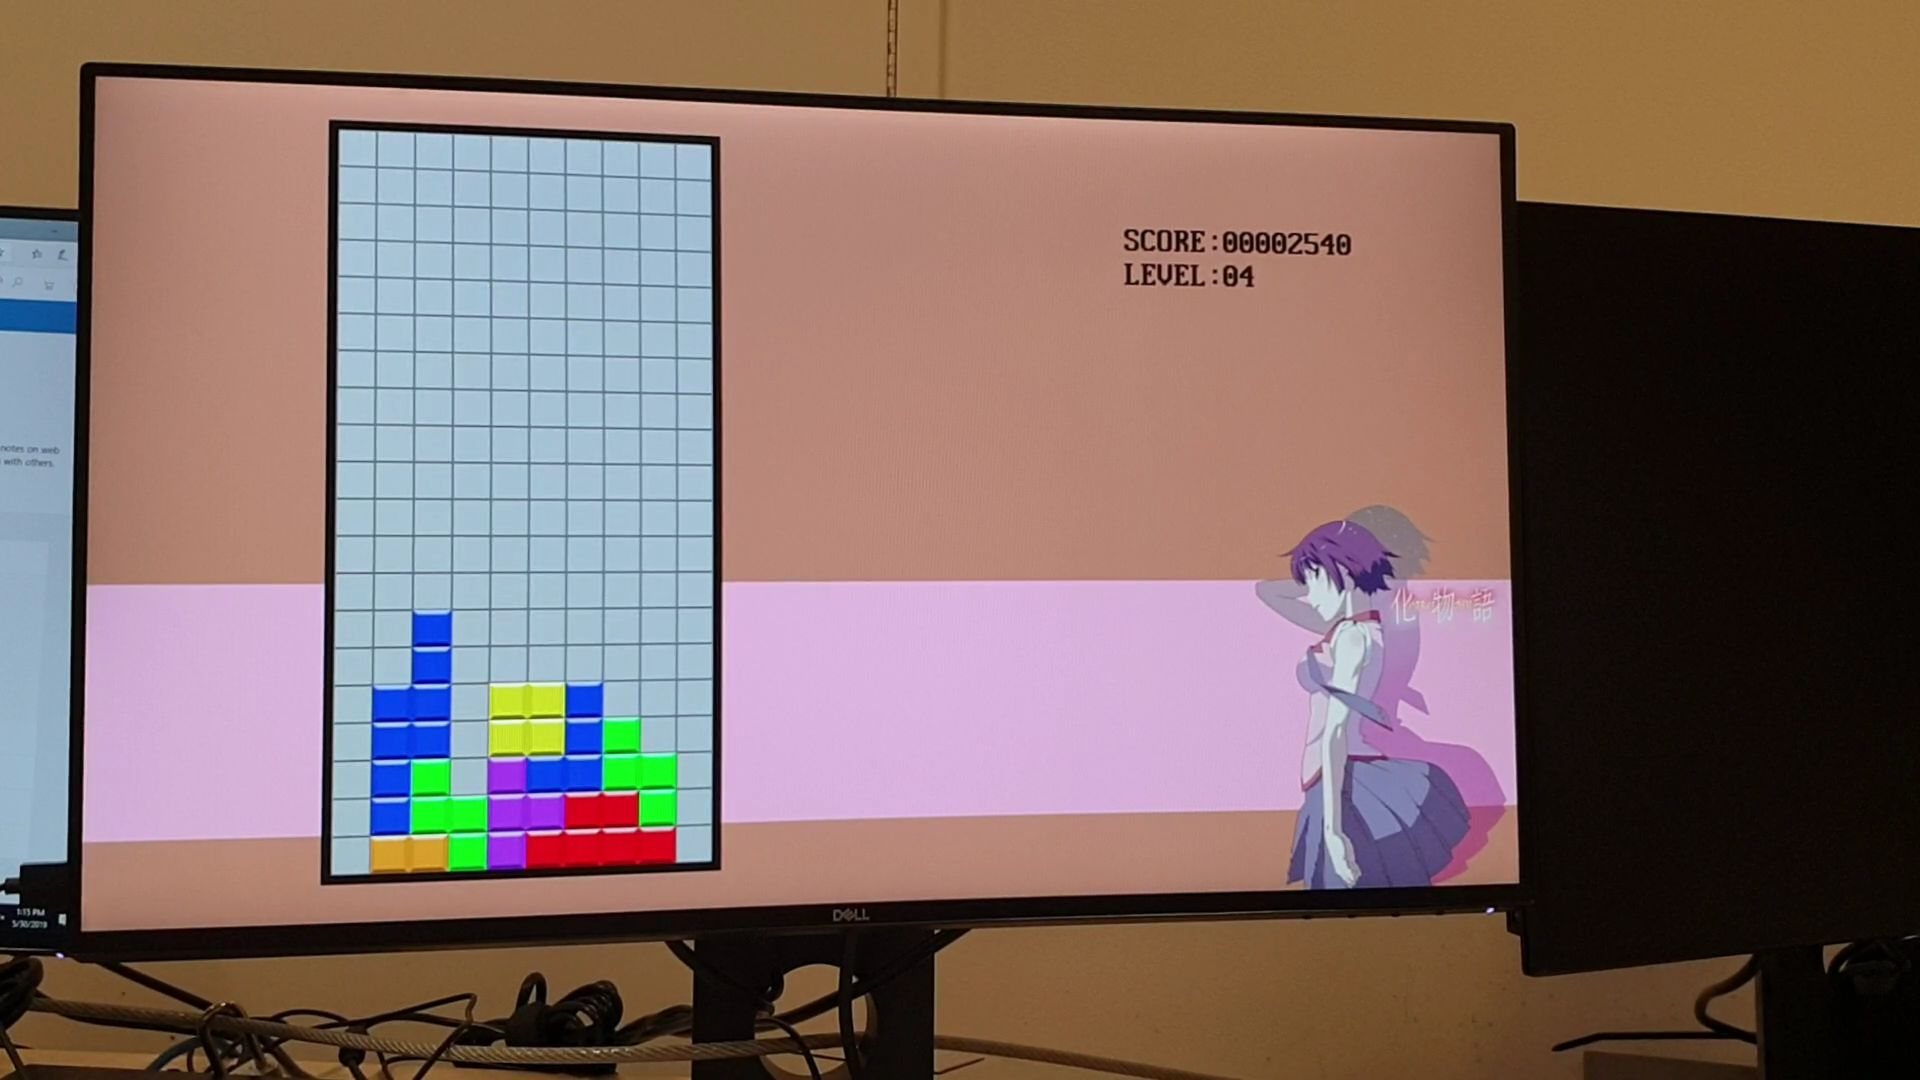
\includegraphics[width=\textwidth]{result.png}
    \caption{Result}\label{result}
  \end{center}
\end{figure}

\subsection{Flow summary}
I optimized stuff by using one \code{check\_valid} for multiple tetris, which use the most
ALUTs (around 1500). Did not know the end result would not use that many ALUTs. May reduce
chance of metastability even further by adding more check\_valid module, but since there was
no problem, I left it be.
\begin{figure}[H]
  \begin{center}
    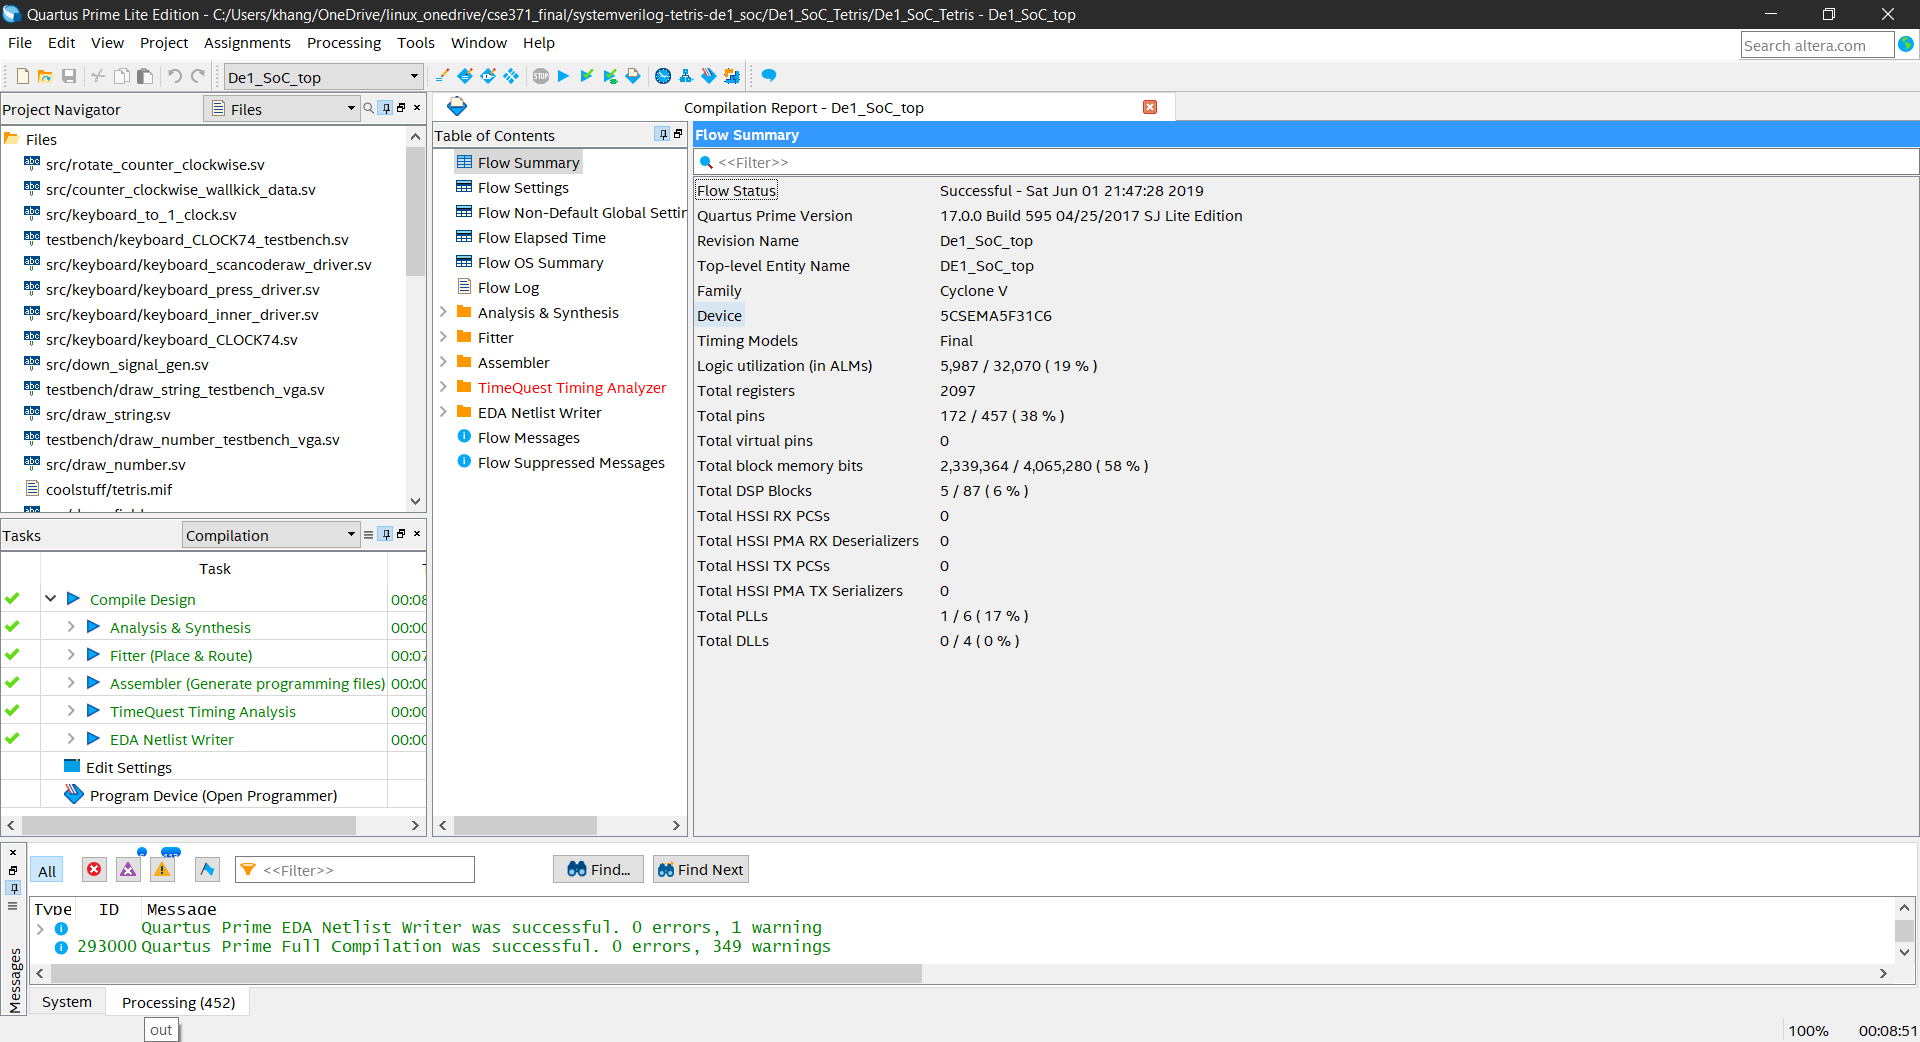
\includegraphics[width=\textwidth]{flow_summary.png}
    \caption{Flow summary}\label{flow_summary}
  \end{center}
\end{figure}

%----------------------------------------------------------------------------------------
%	SECTION 4
%----------------------------------------------------------------------------------------

\section{Problem face and discussion}

You may wonder how the image was converted into rom. First, I convert the image into .bmp
format (bitmap). In the process I found out two thing: the number of pixel of each row will
be round to the nearest multiply of 4 and the pixel start from bottom left instead of top
left. Thus, I invert the image horizontally, open the .bmp file with an hex editor and copy
the hex byte format of the image. When copy to notepad, the format is hex bytes separated
with a space each byte and order is green - red - blue. I use notepad++ to replace regex, convert it
to red - geen - blue, with no space between each three byte, each of them separated with newline.
After that, I append the number from 0 to number of pixel at the begin and
`;' at the end of each line to create a .mif format memory file, which is then read into a ROM.

Second thing I did to improve visual is make the screen display 1280x720p instead of 640x480p.
I was able to find in Altera's DE1-SoC CD a verilog file that have display timing that I can change.
Which I changed into the 1280x720 timing I found online.
Then I use PLL to generate a 74.25 Mhz clock to be used with the display. I also edit the module
so it input 24 bit  color and output VGA\_GREEN/RED/BLUE. Initially, the output VGA\_CLK is invert
of CLOCK\_74 input and caused some undesired artifact, so I change it to CLOCK\_74 directly. Every
other module have to use CLOCK\_74 now.

Now I face a new problem, the keyboard module provided works on CLOCK\_50, not CLOCK\_74, so I created
a FIFO buffer to create \code{keyboard\_CLOCK74} module. It just a FIFO with slower write clock. This
worked with no issue.
\end{document}
